% Thinking Costs Calibration in Diffusion Decision Models.
% DRAFT prose written by the drafting assistant for Aman's review. Every number and claim traces to
% results/CLAIMS.md or a results file; see paper/CLAIM_AUDIT.md. Tables are generated by
% paper/make_tables.py and figures by paper/make_figures.py (do not edit them by hand).
\documentclass[11pt]{article}
\usepackage[margin=1in]{geometry}
\usepackage[utf8]{inputenc}
\usepackage[T1]{fontenc}
\usepackage{amsmath,amssymb}
\usepackage{booktabs}
\usepackage{graphicx}
\usepackage{hyperref}
\usepackage{xurl}
\usepackage[numbers,sort&compress]{natbib}
\usepackage{xcolor}
% generated from results/hypothesis_tests.json
\newcommand{\verdictHone}{supported}
\newcommand{\verdictHtwo}{not supported}
\newcommand{\verdictHthree}{not supported}
\newcommand{\verdictHfour}{supported}


\title{Thinking Costs Calibration in Diffusion Decision Models}
\author{Shaik Aman\\ Independent Researcher\\ \texttt{amanabdul21@gmail.com} \and Jeykumar Chinnathambi\\ Independent Researcher}
\date{}

\begin{document}
\maketitle

\begin{abstract}
System One decision models answer typed questions in a single pass and return probabilities that downstream software acts on.
Masked diffusion language models can serve as such models, and they come with a built-in thinking dial: a scratch region before the answer slot, and the number of denoising steps used to fill it.
We ask whether turning this dial buys better decisions, and what it does to calibration.
We evaluate LLaDA-8B-Instruct on 3,600 test items across four datasets under pre-registered hypotheses, and repeat key conditions on Dream-v0-Instruct-7B.
Adding scratch worsened calibration relative to the single read in 45 of 48 LLaDA settings and 23 of 24 Dream settings.
Accuracy effects depended on the model: deliberation gave LLaDA no consistent gain, while Dream improved with more steps on three of four datasets.
For LLaDA, miscalibration grew with denoising steps and plateaued by 16 steps, and a margin-based escalation rule did not beat fixed budgets.
In an exploratory analysis, deliberation fixed significantly more answers than it broke in only 4 of 48 LLaDA settings, and broke more than it fixed in 16.
Temperature scaling fit per budget recovered much of the lost calibration on average, though not in every setting.
Finally, the single read of both diffusion models was better calibrated than instruction-tuned autoregressive baselines, but Dream's calibration matched its own base model on three of four datasets, which suggests that this gap reflects post-training rather than the diffusion architecture.
\end{abstract}

\section{Introduction}
\label{sec:intro}
A System One decision model reads a state and returns a typed answer with calibrated probabilities that software can use directly \citep{typesafe2026jev}.
In such systems the probability is not a side output. Software uses it to decide whether to act, wait, or ask a person.
A model that is right 70\% of the time but reports 95\% confidence will skip checks it should have triggered.
Calibration therefore matters alongside accuracy.

For autoregressive (AR) language models, more reasoning does not reliably produce better confidence.
Larger reasoning budgets can make models overconfident \citep{hiremath2026calibrationdrift,lacombe2025overreasoning}, and a decision token after reasoning can mainly extract the conclusion of the reasoning trace rather than carry confidence information \citep{yaldiz2026calibrationrl}.
Reasoning-induced overconfidence is therefore already documented for AR models.

Masked diffusion language models can also serve as decision models: the answer is read from a masked slot in a single denoising pass \citep{mastrac2026djev,mastrac2026vllmpr}.
They also offer a dial that AR models do not: a masked scratch region placed before the answer slot, and the number of denoising steps used to fill it.
We found no study of what this dial does to the calibration of typed decisions.

We measure it.
We read a lettered answer from one masked slot of LLaDA-8B-Instruct \citep{nie2025llada} under a single read (C0), with a scratch region that is denoised while the answer template is visible (C1), and with a pre-read thought that is denoised without the template and then followed by the answer (C2).
We vary the scratch length $S$ and the number of steps $T$ on 3,600 test items from four datasets, and repeat key conditions on Dream-v0-Instruct-7B \citep{ye2025dream}.

Our contributions are:
\begin{itemize}
  \item A pre-registered measurement of accuracy and calibration across a thinking dial in a diffusion decision model. Two of four pre-registered hypotheses were supported.
  \item Evidence that adding scratch worsens calibration relative to the single read for both models tested, and that temperature scaling fit per budget recovers much of the loss on average.
  \item An analysis, exploratory, of why a confidence-margin escalation rule does not beat fixed budgets: deliberation flips answers in both directions, and fixes significantly more than it breaks in only 4 of 48 settings.
  \item A comparison, exploratory, of the single read against AR models, showing that the calibration gap to instruction-tuned AR models largely disappears against Dream's own base model.
\end{itemize}
Our main result extends a known AR effect to a new model family and readout. It is a measurement, not a new method.
All hypotheses, splits, and analysis rules were frozen before the test set was run.
Analyses added after the test results are labeled exploratory throughout.

\section{Related Work}
\label{sec:related}
\paragraph{System One decision models.}
TypeSafe describes System One models as models ``built to make fast, structured decisions that software can use directly'', with answers ``accompanied with calibrated probabilities'' \citep{typesafe2026jev}.
Laya's model card describes it as a ``multilingual, non-autoregressive System 1 decision model''; its main checkpoint uses a ModernBERT-large encoder and its multilingual checkpoint uses mmBERT-base \citep{convai2026laya}.
CLM-8B places a state head and an action head on a frozen Qwen3-8B encoder, trained with a bidirectional InfoNCE loss \citep{contrastivelm2026clm}.
djev reads typed decisions from DiffusionGemma by seeding a canvas with the answer's fixed text and reading the noised answer slots after one denoise step, with an optional thought channel written before the read \citep{mastrac2026djev}; the serving support was merged into vLLM \citep{mastrac2026vllmpr}.
None of these sources reports a calibration sweep over scratch length or denoising steps.

\paragraph{Diffusion language models.}
LLaDA is a masked diffusion model trained from scratch with pre-training and supervised fine-tuning \citep{nie2025llada}.
Dream 7B is a discrete diffusion model whose training uses AR-based LLM initialization \citep{ye2025dream}.
A systematic comparison of eight diffusion models finds that their behavior depends strongly on generation-time choices such as denoising steps \citep{bertolani2026dlmanalysis}.

\paragraph{Reasoning and calibration in AR models.}
Calibration Drift Under Reasoning reports that ECE can first decrease and then increase as the reasoning budget grows, with an 8B model becoming overconfident \citep{hiremath2026calibrationdrift}.
On expert-confidence assessment, larger reasoning budgets consistently impaired calibration \citep{lacombe2025overreasoning}.
RLVR fine-tuning produced overconfident decision models, which a calibration-aware RL objective mitigated; the same work argues that a decision token after reasoning mainly extracts the conclusion of the reasoning trace and does not carry confidence information \citep{yaldiz2026calibrationrl}.
The shape of the entropy trajectory during chain-of-thought predicts reasoning reliability \citep{zhao2026entropytrajectory}.
These works study AR models.
We study the analogous question in diffusion decision models.

\paragraph{Calibration and decoding dynamics in diffusion LMs.}
On masked WikiText infilling with LLaDA-8B-Base, late confidence becomes less calibrated even though uncertainty stays higher for tokens that resolve incorrectly \citep{lu2026temporal}.
Diffusion models can encode input errors internally while their reported confidence stays near its maximum under noise \citep{yadav2026unsure}.
A paired comparison including Dream-7B and Qwen2.5-7B reports systematic overconfidence in diffusion models \citep{yadav2026bidirectional}.
Prophet observes that answers often converge before the final step and stops decoding early using the top-2 confidence gap \citep{li2025prophet}.
Delaying a reserved answer position can improve accuracy over an equally timed reasoning-token delay \citep{yeom2026answerfirst}.
In-place chain-of-thought prompting inside masked positions, with a confidence-aware early exit, improves accuracy and speed \citep{jin2025thinkinginsidemask}.
Our margin-based escalation rule uses the same top-2 gap as Prophet, but applies it to typed decisions and evaluates calibration.

\paragraph{Unmasking order.}
LogicDiff replaces confidence-based unmasking with logic-role-guided unmasking and improves zero-shot reasoning in LLaDA-8B-Instruct \citep{aman2026logicdiff}.
We use confidence-based unmasking throughout and leave scheduling variants to future work.

\section{Setup}
\label{sec:setup}
\paragraph{Models.}
The primary model is LLaDA-8B-Instruct (revision 08b83a6). The second diffusion model is Dream-v0-Instruct-7B (revision 05334cb), whose logits are shifted right by one position as in its own generation code. AR baselines are Qwen3-8B \citep{yang2025qwen3} and, for one exploratory comparison, Qwen2.5-7B-Instruct (revision a09a354) and Qwen2.5-7B base (revision d149729) \citep{yang2024qwen25}. All runs use bf16, batch size 1, and greedy decoding on one NVIDIA L4 GPU.

\paragraph{Canvases.}
Each item is rendered as lettered multiple choice with shuffled options. The user prompt ends with: \emph{If you have space to think, think step by step first. Then finish with ``The answer is'' followed by the letter.}
C0 appends \texttt{The answer is}, one masked slot, and an end-of-turn token (\texttt{<|eot\_id|>} for LLaDA, \texttt{<|im\_end|>} for Dream).
C1 appends \texttt{Let me think step by step.}, a newline, $S$ masked scratch tokens, a newline, \texttt{The answer is}, the slot, and the end-of-turn token. Scratch positions are unmasked by confidence over $T$ steps; the slot is never written and is read after the last step.
C2 denoises \texttt{Let me think step by step.} followed by $S$ masks with no answer template or slot visible, then appends the template, slot, and end-of-turn token and reads once.
The slot distribution is a softmax over letters, each scored by the logsumexp of its single-token variants. Off-label mass is the full-vocabulary probability outside these variants.
The grid is C0 plus C1 and C2 at $S\in\{32, 128\}$ and $T\in\{1, 4, 16\}$: 13 cells. A C1 or C2 cell costs $T{+}1$ forward passes (NFE).

\paragraph{Data.}
We use BoolQ \citep{clark2019boolq}, StrategyQA \citep{geva2021strategyqa}, ARC-Challenge \citep{clark2018arc}, and a synthetic ``jagged'' set of counting, date comparison, indirection, and decimal comparison items (Table~\ref{tab:data}). BoolQ passages are truncated to 300 words. Option order is shuffled per item with a stable hash of the item id. Items were split into dev and test once, by seed. Exploratory runs on Dream and the Qwen2.5 models use the original test subset.
% generated by paper/make_tables.py from results/splits.json
\begin{table}[t]
\centering
\small
\caption{Items per split. Test is the original (v1.1) test set plus seed-drawn additions registered before test (v1.2).}
\label{tab:data}
\begin{tabular}{llrr}
\toprule
Dataset & Dev & Test & Test (original) \\
\midrule
BoolQ & 100 & 1000 & 400 \\
StrategyQA & 100 & 1000 & 400 \\
ARC-C & 100 & 1000 & 400 \\
Jagged & 60 & 600 & 240 \\
\bottomrule
\end{tabular}
\end{table}


\paragraph{Metrics and statistics.}
We report accuracy, ECE with 15 equal-width bins \citep{guo2017calibration}, adaptive ECE with 15 equal-mass bins \citep{nixon2019measuring}, Brier score, NLL, AURC \citep{geifman2017selective}, and off-label mass. Temperature scaling \citep{guo2017calibration} fits one temperature per model and cell on dev by NLL; a secondary variant fits one per dataset and cell. Differences use a paired bootstrap over items (1000 resamples, seed 1234, 95\% percentile intervals) and McNemar's exact test for accuracy.

\paragraph{Escalation.}
The pre-registered ladder runs C0, then C1($S{=}32,T{=}4$), then C1($S{=}128,T{=}16$), escalating while the top-2 margin is below a threshold $\tau$ (cumulative NFE 1, 6, 23). For each dataset we sweep 50 values of $\tau$ in $[0,1]$ and compute $G$, the mean gap between escalation accuracy and the fixed-budget frontier (the running maximum of fixed-cell accuracy over NFE). The escalation curve dominates the frontier on a dataset if the confidence interval of $G$ lies above 0.

\paragraph{Protocol history.}
A first smoke run (v1.0) on 20 dev items per dataset found that the answer slot, as the last position of the sequence, put most of its mass outside the letters (median off-label mass 0.989), and that the pre-read thought only restated an answer. Before any dev data was used, protocol v1.1 pinned the end-of-turn token after the slot, added the step-by-step prefix, and changed the last prompt line; median off-label mass fell to 0.016. Hypotheses H1 to H4 were unchanged. Before the test set was run, v1.2 registered the full-curve H3 test, adaptive ECE, per-dataset temperature scaling, an end-token ablation, and an expanded test set. A pre-registered check on 50 dev items found that reading the slot after step 4 of a $T{=}16$ run is not equivalent to a native $T{=}4$ run (argmax agreement 0.90, ECE difference 0.027), so every budget was run natively. Analyses in v1.3 and v1.4 were added after the test results and are exploratory. All runs used 23.67 instance-hours on an AWS g6.2xlarge.

\section{Results}
\label{sec:results}
Table~\ref{tab:hyp_summary} summarizes the pre-registered tests on LLaDA-8B-Instruct.
% generated by paper/make_tables.py from results/hypothesis_tests.json
\begin{table}[t]
\centering
\small
\caption{Pre-registered hypotheses (LLaDA-8B-Instruct, test set). Full contrasts in Appendix Table~\ref{tab:hypotheses}.}
\label{tab:hyp_summary}
\resizebox{\linewidth}{!}{%
\begin{tabular}{llrrr}
\toprule
H & Contrast & Verdict & Calls & Estimate range \\
\midrule
H1 & C1 ECE($T{=}16$) $-$ ECE($T{=}1$), 4 datasets $\times$ $S\in\{32,128\}$ & supported & 8/8 CIs $>0$ & 0.058 to 0.161 \\
H2 & Acc C1($S{=}128,T{=}16$) $-$ Acc C0 & not supported & BoolQ met; StrategyQA inconcl.; ARC-C met; Jagged failed & -0.113 to 0.027 \\
H3 & Mean gap $G$, escalation curve vs fixed frontier & not supported & 0/4 dominate & -0.039 to 0.001 \\
H4 & C1 $-$ C2 (Acc, ECE) at $S{=}128$, $T{=}16$ & supported & 3/8 CIs exclude 0 & -0.043 to 0.048 \\
\bottomrule
\end{tabular}}
\end{table}


\paragraph{H1 (pre-registered, supported; LLaDA only).}
At fixed scratch length, raw ECE of the answer slot rose from $T{=}1$ to $T{=}16$ in C1. All 8 contrasts (four datasets, two scratch lengths) had confidence intervals above 0, with estimates from 0.058 to 0.161. Accuracy did not move with it: 6 of the 8 accuracy contrasts included 0, one was positive (StrategyQA, $S{=}128$: 0.041 [0.006, 0.075]), and one was negative (jagged, $S{=}128$: $-$0.030 [$-$0.057, $-$0.002]).

\paragraph{H2 (pre-registered, not supported; LLaDA only).}
We predicted that scratch would help on StrategyQA and jagged but not on BoolQ or ARC-C. For C1($S{=}128,T{=}16$) against C0, StrategyQA gained 0.027 [$-$0.001, 0.054] (inconclusive), and jagged lost 0.113 [$-$0.150, $-$0.075]. BoolQ changed by $-$0.036 [$-$0.056, $-$0.015], a significant loss, and ARC-C by $-$0.018 [$-$0.038, 0.000]. Under the registered rule these last two count as ``no gain''.

\paragraph{H3 (pre-registered, not supported; LLaDA only).}
The escalation curve did not dominate the fixed-budget frontier on any dataset. $G$ was $-$0.001 on BoolQ, $-$0.008 on StrategyQA, 0.001 on ARC-C, and $-$0.039 [$-$0.069, $-$0.019] on jagged, where the curve fell below the frontier (Appendix Table~\ref{tab:h3}). A second, dev-selected ladder ending at C1($S{=}32,T{=}16$), labeled exploratory, also failed (Appendix Table~\ref{tab:escalation}; Figure~\ref{fig:acc_nfe}).

\paragraph{H4 (pre-registered, supported; LLaDA only).}
In-canvas scratch and pre-read thought differed at $S{=}128$, $T{=}16$. Where they differed, C2 was better: accuracy differences (C1 minus C2) were $-$0.030 [$-$0.048, $-$0.013] on BoolQ and $-$0.043 [$-$0.073, $-$0.015] on jagged, and the ECE difference was 0.048 [0.018, 0.079] on jagged. The other five contrasts included 0.

\paragraph{Any scratch versus none (exploratory).}
In almost every cell, adding scratch worsened calibration relative to C0. The ECE difference had a confidence interval above 0 in 45 of 48 LLaDA cells on the full test set and in 23 of 24 Dream cells on the original test items (Appendix Table~\ref{tab:anythinking}; Figure~\ref{fig:calibration_summary}). Figure~\ref{fig:reliability} shows the same pattern in reliability diagrams for C0 and C1($S{=}128,T{=}16$).

\paragraph{Temperature scaling (exploratory aggregate).}
Over the 48 LLaDA scratch cells, mean ECE was 0.191 raw, 0.096 after one temperature per cell (a 50\% reduction), and 0.060 after one temperature per dataset and cell (68\%). These lowered ECE in 88\% and 90\% of cells. For Dream, mean scratch ECE fell from 0.182 to 0.111 with its own dev temperatures. Scaling did not always help: it raised Dream's mean scratch ECE on ARC-C from 0.117 to 0.128, raised Dream's C0 ECE on BoolQ, ARC-C, and jagged, raised LLaDA's C0 ECE on ARC-C from 0.048 to 0.055, and raised Qwen3-8B's C0 ECE on ARC-C from 0.078 to 0.203.

\paragraph{End-token suppression (registered secondary ablation; LLaDA only).}
At $S{=}128$, C2 thoughts sometimes ended early with end-of-text tokens (median share up to 0.50 on StrategyQA). Blocking these tokens in scratch positions changed nothing in C1, whose scratch contained none. In C2 it did not change accuracy significantly, but it worsened calibration: ECE rose by 0.103 [0.062, 0.128] on StrategyQA at $T{=}1$, by 0.074 [0.037, 0.108] at $T{=}4$, and by 0.037 at $T{=}16$, and by 0.042 [0.006, 0.061] on jagged at $T{=}4$ (Appendix~\ref{app:tables}). Forcing longer thoughts did not help.

\begin{figure}[t]
\centering
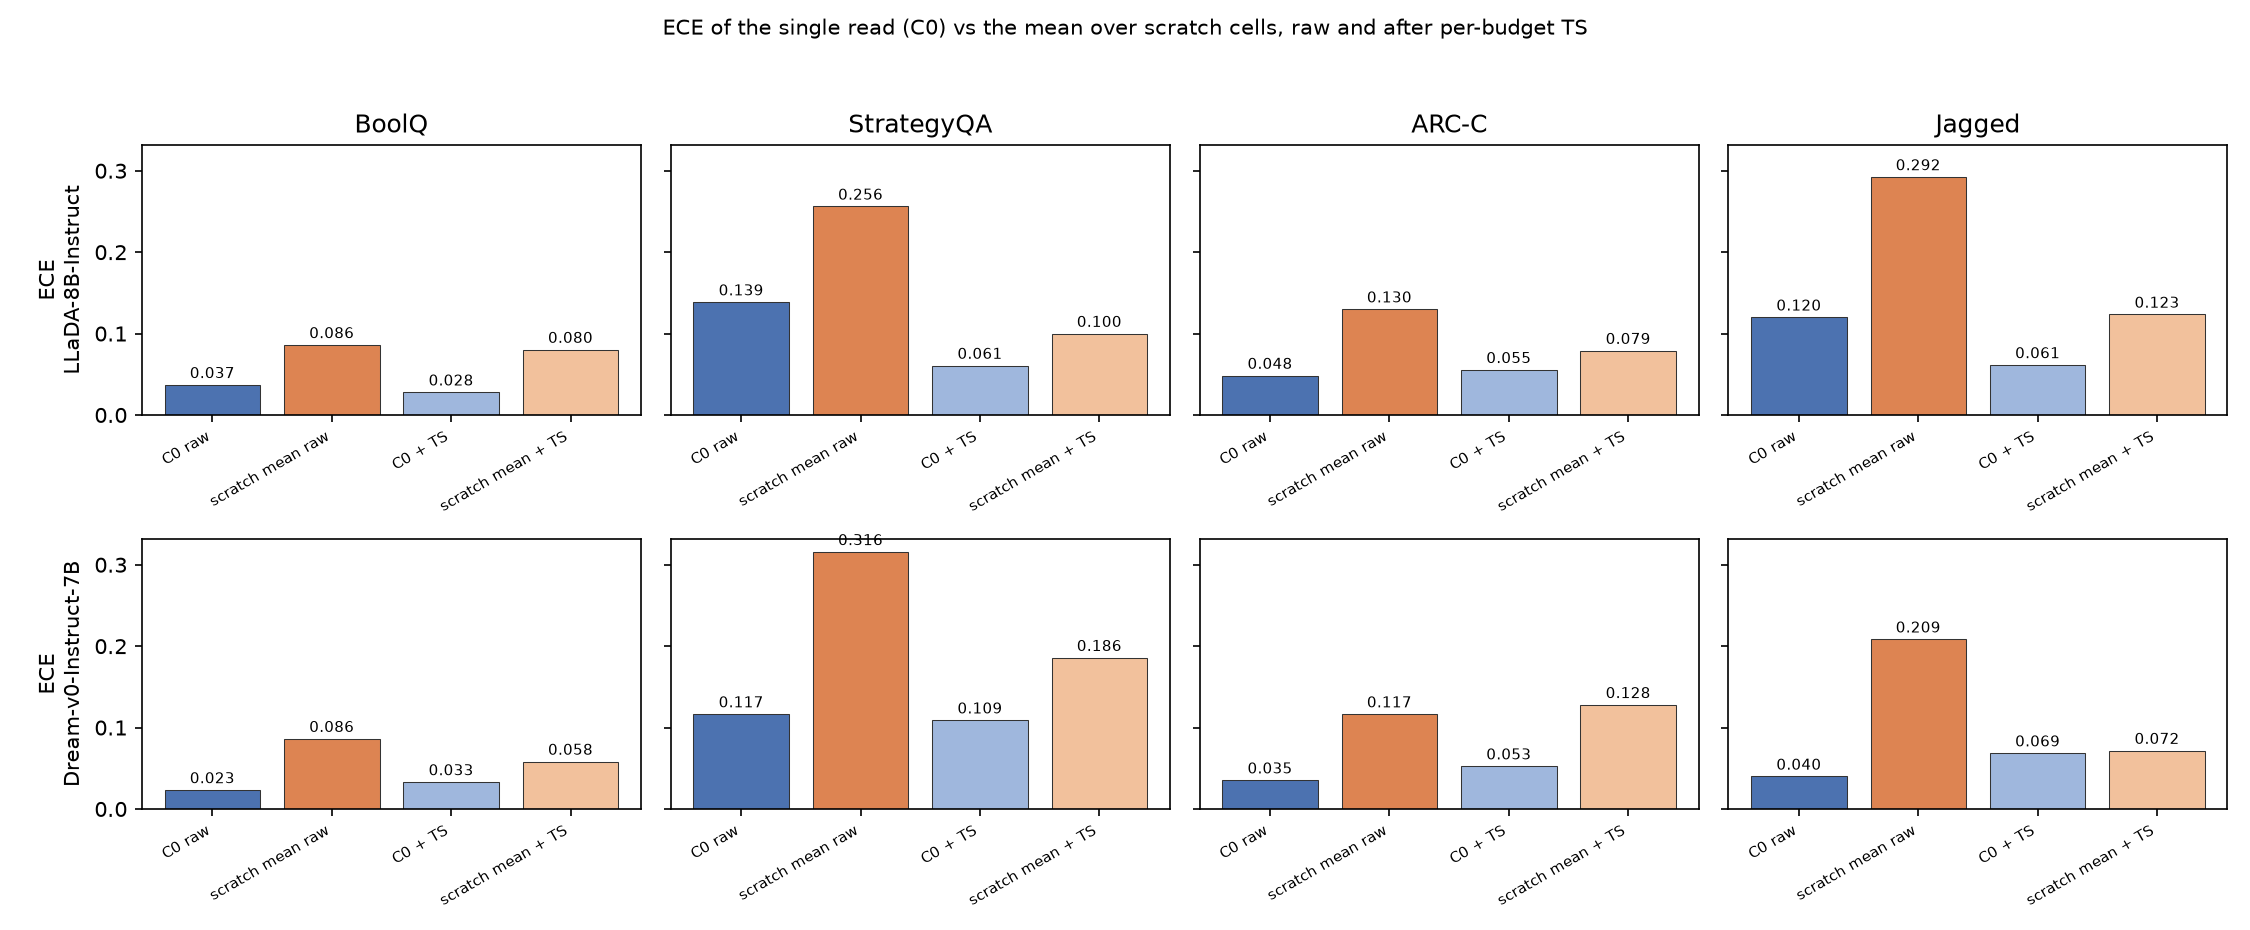
\includegraphics[width=\linewidth]{figs/calibration_summary.png}
\caption{ECE of the single read (C0) and the mean ECE over scratch cells, raw and after per-budget temperature scaling (one temperature per cell, fit on dev). Top: LLaDA-8B-Instruct, full test set, 12 scratch cells. Bottom: Dream-v0-Instruct-7B, original test items, 6 scratch cells. Raw scratch ECE exceeds C0 ECE for every dataset and both models; scaling narrows the gap on average but not everywhere.}
\label{fig:calibration_summary}
\end{figure}

\section{Analysis (exploratory)}
\label{sec:analysis}
Everything in this section was added after the test results were seen.

\paragraph{Miscalibration plateaus by 16 steps (LLaDA only).}
On the original test items at $S{=}32$, ECE at $T{=}32$ (one token per step) exceeded ECE at $T{=}1$ in all 8 condition and dataset pairs, and did not differ from ECE at $T{=}16$ in any of them. Accuracy at $T{=}32$ did not differ from $T{=}1$ in any pair (Appendix Table~\ref{tab:t32}). Figure~\ref{fig:ece_nfe} shows raw ECE against NFE for all fixed cells.

\begin{figure}[t]
\centering
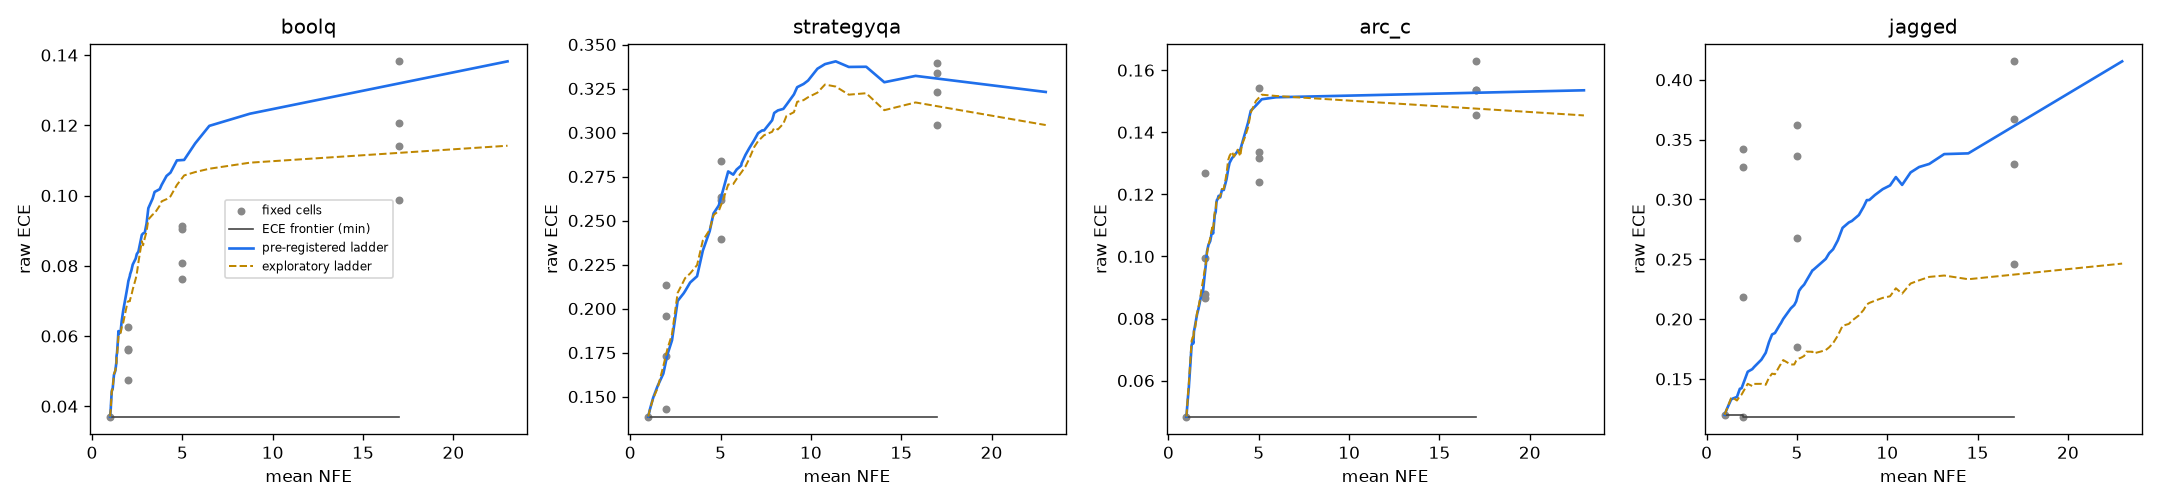
\includegraphics[width=\linewidth]{figs/ece_vs_nfe_test.png}
\caption{Raw ECE against mean NFE for LLaDA-8B-Instruct on the full test set: fixed cells, the lowest-ECE frontier, and both escalation ladders. The ECE of both ladders rises as they spend more forward passes, and most scratch cells sit above C0.}
\label{fig:ece_nfe}
\end{figure}

\paragraph{Why escalation fails (LLaDA only).}
The C0 margin does identify fixable items. Among items wrong at C0, the AUROC of the negative margin for predicting that C1($S{=}32,T{=}16$) is correct ranged from 0.582 to 0.812, though the jagged interval [0.497, 0.665] includes 0.5 (Appendix Table~\ref{tab:margin_auroc}). The problem is churn. Deliberation fixes some items and breaks others. Across the 48 LLaDA scratch cells, the net change (fixed minus broken, as a share of items) had a confidence interval above 0 in 4 cells, below 0 in 16, and including 0 in 28. For example, on StrategyQA, C1($S{=}32,T{=}16$) turned 134 wrong answers right and 99 right answers wrong; on jagged, C1($S{=}128,T{=}16$) did 37 and 105 (Appendix Table~\ref{tab:flips}). If an escalated answer must be correct in both C1 and C2 at that budget, only 42\% to 54\% of the pre-registered ladder's oracle headroom remains (Appendix Table~\ref{tab:oracle_stability}).

\paragraph{Stated answers (LLaDA only).}
The two scratch modes behave differently. At $T{=}16$, C2 thoughts stated an explicit answer in 96.4\% to 100\% of items, and the slot agreed with that answer in over 99\% of them. This fits the view that a decision read after reasoning mainly extracts the conclusion of the reasoning \citep{yaldiz2026calibrationrl}.
C1 does not fit that view. Its scratch stated an explicit answer in at most 2.7\% of items (ARC-C at $S{=}128$ is the exception, at 15.4\%), yet its confidence still rose. At $S{=}32$, $T{=}16$, the mean top-1 probability of items that ended correct rose from 0.765 to 0.936 at the first readout to 0.939 to 0.987 at the final read, and that of items that ended wrong rose from 0.714 to 0.797 to 0.876 to 0.939. Wrong items gained confidence about as fast as correct ones, so confidence separated them less well as steps increased (Figure~\ref{fig:anytime}). We do not identify what drives this rise in C1; answer detection used a regular expression and may miss implicit answers.

\paragraph{Dream differs from LLaDA.}
Table~\ref{tab:dream_compact} summarizes Dream. Unlike LLaDA, Dream gained accuracy with more steps in C1 at $S{=}32$: 0.055 [0.025, 0.088] on BoolQ, 0.075 [0.025, 0.125] on StrategyQA, and 0.104 [0.058, 0.158] on jagged ($T{=}16$ minus $T{=}1$). Its ECE did not rise consistently with steps: the difference was 0.046 on ARC-C, $-$0.043 on jagged, and included 0 on the other two datasets. For Dream, the larger calibration cost came from adding any scratch at all. The C1 versus C2 direction also differed: on jagged, C1 was more accurate (0.067 [0.017, 0.121]) and better calibrated ($-$0.072 [$-$0.116, $-$0.013]); on StrategyQA, C2 was more accurate ($-$0.043 [$-$0.085, $-$0.005]) (Appendix Table~\ref{tab:dream_contrasts}). Dream was tested only at $S{=}32$ and on the original test items.
% generated by paper/make_tables.py from results/v13_bc.json
\begin{table}[t]
\centering
\small
\caption{Dream-v0-Instruct-7B (exploratory, original test items): accuracy / ECE for C0 and selected $S{=}32$ cells. Full table in Appendix Table~\ref{tab:dream}.}
\label{tab:dream_compact}
\begin{tabular}{llrrr}
\toprule
Dataset & C0 & C1 $T{=}1$ & C1 $T{=}16$ & C2 $T{=}16$ \\
\midrule
BoolQ & 0.910 / 0.023 & 0.843 / 0.085 & 0.897 / 0.094 & 0.892 / 0.097 \\
StrategyQA & 0.613 / 0.117 & 0.557 / 0.324 & 0.632 / 0.300 & 0.675 / 0.314 \\
ARC-C & 0.870 / 0.035 & 0.863 / 0.084 & 0.860 / 0.129 & 0.877 / 0.119 \\
Jagged & 0.729 / 0.040 & 0.725 / 0.196 & 0.829 / 0.153 & 0.762 / 0.225 \\
\bottomrule
\end{tabular}
\end{table}


\paragraph{The single read against AR models.}
This comparison is context, not a claim that diffusion models are better calibrated. On the full test set, LLaDA's C0 ECE was lower than Qwen3-8B's on all four datasets (differences from $-$0.150 to $-$0.029), while its accuracy was lower on StrategyQA ($-$0.062) and ARC-C ($-$0.053). On the original test items, C0 ECE was lower than Qwen2.5-7B-Instruct's for Dream ($-$0.228 to $-$0.071) and for LLaDA ($-$0.187 to $-$0.053), with accuracy differences whose intervals included 0. Dream was initialized from Qwen2.5-7B base, not from the Instruct model. Against that base model, Dream's ECE difference included 0 on BoolQ, StrategyQA, and ARC-C and was $-$0.077 [$-$0.118, $-$0.004] on jagged (Appendix Tables~\ref{tab:onepass_a} and \ref{tab:onepass_b}). The dev-fitted C0 temperatures were 5.79 for Qwen2.5-7B-Instruct, 1.63 for Qwen2.5-7B base, and 1.05 for Dream. This pattern is consistent with post-training, rather than architecture, driving the gap. It rests on one model pair, the base model was prompted with a chat template, and post-training is confounded with architecture.
A paired study reports systematic overconfidence in diffusion models relative to AR models \citep{yadav2026bidirectional}. Our single-slot readout and evaluation differ from theirs, so we do not read our results as contradicting that finding; they show only that, in our setting, the single read of an instruction-tuned diffusion model was not more overconfident than its AR relatives.

\section{Discussion}
\label{sec:discussion}
Our results extend a pattern known from AR models to diffusion decision models, with one difference in where the cost appears. In AR models, longer reasoning budgets have been linked to overconfidence \citep{hiremath2026calibrationdrift,lacombe2025overreasoning}. In both diffusion models we tested, the cost appeared as soon as any scratch was added. In LLaDA it then grew with denoising steps and plateaued by 16 steps. In Dream it did not grow consistently with steps, while accuracy did.

For builders who read decisions from a diffusion model, three points follow. First, the single read had lower raw ECE than almost every scratch cell in both models; the one exception was LLaDA's C1($S{=}32,T{=}1$) on jagged. Adding scratch should not be assumed to make the probabilities more trustworthy, even when it improves accuracy, as it did for Dream. Second, if scratch is used, the temperature should be refit for each budget and checked per dataset. On average this recovered much of the calibration loss, but it raised ECE in some cells. Third, confidence-based escalation should be tested before it is relied on. For LLaDA, the C0 margin did identify fixable items, but deliberation broke about as many correct answers as it fixed, so escalation did not beat a fixed budget.

The two scratch modes point to different mechanisms. In C2, the slot almost always repeated an answer the thought had already stated, which fits the extraction view from AR work \citep{yaldiz2026calibrationrl}, although our prompt encouraged this pattern. In C1, confidence rose even though the scratch rarely stated an answer, and items that ended wrong gained confidence about as fast as items that ended correct. We do not know what drives this. One possibility is that committed scratch tokens sharpen the slot distribution through bidirectional attention regardless of their content; we did not test this.

Some findings held for both models and some did not. The calibration cost of adding scratch, and the average benefit of per-budget temperature scaling, appeared in both LLaDA and Dream. The growth of miscalibration with steps (H1), the plateau by 16 steps, and the advantage of pre-read thought (H4) were shown for LLaDA only, and Dream behaved differently on steps and on the C1 versus C2 direction. Two diffusion models are not enough to say which of these behaviors is typical of the model class.

Several questions remain open. We tested only confidence-ordered unmasking; scheduling methods such as LogicDiff \citep{aman2026logicdiff} change which scratch tokens are committed first and may change both accuracy and calibration. We tested greedy decoding only, and Dream only at $S{=}32$. Larger scratch budgets, sampling, more diffusion models, System One models built on DiffusionGemma \citep{mastrac2026djev}, and training objectives that target calibration under deliberation \citep{yaldiz2026calibrationrl} are natural next steps.

\section{Limitations}
\label{sec:limitations}
Several results rest on one model. H1, the direction of H4, the plateau by 16 steps, the churn explanation of H3, the stated-answer behavior of C1 and C2, the end-token ablation, and the anytime-readout check were shown for LLaDA-8B-Instruct only, and the direction of H4 reverses for Dream on jagged.
Dream-v0-Instruct-7B was run only at $S{=}32$ with $T\in\{1, 4, 16\}$ and only on the original test items (400, 400, 400, and 240 items).
The comparison with Qwen2.5-7B base uses one model pair, prompts the base model with a chat template, and cannot separate the post-training recipe from the architecture.
StrategyQA items come from its train split, the only labeled split, so they may appear in pretraining data.
The jagged items are synthetic.
All decoding is greedy.
All items are in English.
Every analysis added after the test results (v1.3 and v1.4) is exploratory.
We applied no correction for multiple comparisons; counts across cells, such as 45 of 48, are exploratory and uncorrected. C2's high rate of stated answers is partly induced by our prompt, which asks the model to finish with ``The answer is''.

\section{Conclusion}
\label{sec:conclusion}
We asked what a thinking dial does to a diffusion decision model.
Adding scratch worsened calibration relative to the single read in nearly every setting for both LLaDA-8B-Instruct and Dream-v0-Instruct-7B, extending to diffusion decision models an effect already documented for AR models.
Whether thinking bought accuracy depended on the model: LLaDA gained little, while Dream improved with more steps.
For LLaDA, miscalibration grew with denoising steps and plateaued by 16 steps, and a margin-based escalation rule did not beat fixed budgets because deliberation flipped answers in both directions.
Temperature scaling fit per budget recovered much of the lost calibration on average.
Two of four pre-registered hypotheses were supported.
For System One models built on diffusion language models, the single read is a strong default, and any added deliberation should come with its own calibration.

\section*{Use of AI tools}
We used AI assistants (Claude Code, Claude, and Cursor) for experiment code, experiment execution, and drafting and editing the text. All results were computed from logged runs, and the authors verified all claims against them.

\section*{Reproducibility}
Code, configurations, per-item outputs, and analysis scripts are available at \url{https://github.com/aman-source/dlm-deliberation}.


\bibliographystyle{plainnat}
\bibliography{refs}

\clearpage
\appendix
\section{Additional tables and figures}
\label{app:tables}
% generated by paper/make_tables.py from results/hypothesis_tests.json
\begin{table}[h!]
\centering
\scriptsize
\caption{All pre-registered contrasts (paired bootstrap, 1000 resamples, 95\% CI; McNemar exact).}
\label{tab:hypotheses}
\resizebox{\linewidth}{!}{%
\begin{tabular}{llrrrr}
\toprule
H & Dataset & Contrast & Estimate [CI] & McNemar p & Call \\
\midrule
H1 & ARC-C & C1 S=32 ECE(T=16) - ECE(T=1) & 0.059 [0.035, 0.076] & -- & supported \\
H1-accuracy & ARC-C & C1 S=32 accuracy(T=16) - accuracy(T=1) & -0.001 [-0.020, 0.018] & 1.0000 & inconclusive \\
H1 & ARC-C & C1 S=128 ECE(T=16) - ECE(T=1) & 0.066 [0.043, 0.082] & -- & supported \\
H1-accuracy & ARC-C & C1 S=128 accuracy(T=16) - accuracy(T=1) & -0.005 [-0.023, 0.014] & 0.6849 & inconclusive \\
H2 & ARC-C & C1(S=128,T=16) accuracy - C0 accuracy & -0.018 [-0.038, 0.000] & 0.0950 & as predicted (no gain) \\
H4 & ARC-C & C1 - C2 accuracy at S=128, T=16 & -0.002 [-0.021, 0.015] & 0.9142 & inconclusive \\
H4 & ARC-C & C1 - C2 ECE at S=128, T=16 & -0.000 [-0.016, 0.020] & -- & inconclusive \\
H1 & BoolQ & C1 S=32 ECE(T=16) - ECE(T=1) & 0.058 [0.036, 0.070] & -- & supported \\
H1-accuracy & BoolQ & C1 S=32 accuracy(T=16) - accuracy(T=1) & 0.000 [-0.016, 0.016] & 1.0000 & inconclusive \\
H1 & BoolQ & C1 S=128 ECE(T=16) - ECE(T=1) & 0.082 [0.055, 0.095] & -- & supported \\
H1-accuracy & BoolQ & C1 S=128 accuracy(T=16) - accuracy(T=1) & -0.011 [-0.033, 0.011] & 0.3712 & inconclusive \\
H2 & BoolQ & C1(S=128,T=16) accuracy - C0 accuracy & -0.036 [-0.056, -0.015] & 0.0004 & as predicted (no gain) \\
H4 & BoolQ & C1 - C2 accuracy at S=128, T=16 & -0.030 [-0.048, -0.013] & 0.0012 & supported \\
H4 & BoolQ & C1 - C2 ECE at S=128, T=16 & 0.017 [-0.002, 0.035] & -- & inconclusive \\
H1 & Jagged & C1 S=32 ECE(T=16) - ECE(T=1) & 0.128 [0.084, 0.159] & -- & supported \\
H1-accuracy & Jagged & C1 S=32 accuracy(T=16) - accuracy(T=1) & -0.023 [-0.058, 0.015] & 0.2504 & inconclusive \\
H1 & Jagged & C1 S=128 ECE(T=16) - ECE(T=1) & 0.074 [0.044, 0.101] & -- & supported \\
H1-accuracy & Jagged & C1 S=128 accuracy(T=16) - accuracy(T=1) & -0.030 [-0.057, -0.002] & 0.0385 & negative \\
H2 & Jagged & C1(S=128,T=16) accuracy - C0 accuracy & -0.113 [-0.150, -0.075] & 0.0000 & not supported \\
H4 & Jagged & C1 - C2 accuracy at S=128, T=16 & -0.043 [-0.073, -0.015] & 0.0049 & supported \\
H4 & Jagged & C1 - C2 ECE at S=128, T=16 & 0.048 [0.018, 0.079] & -- & supported \\
H1 & StrategyQA & C1 S=32 ECE(T=16) - ECE(T=1) & 0.161 [0.130, 0.197] & -- & supported \\
H1-accuracy & StrategyQA & C1 S=32 accuracy(T=16) - accuracy(T=1) & 0.020 [-0.012, 0.051] & 0.2561 & inconclusive \\
H1 & StrategyQA & C1 S=128 ECE(T=16) - ECE(T=1) & 0.150 [0.116, 0.184] & -- & supported \\
H1-accuracy & StrategyQA & C1 S=128 accuracy(T=16) - accuracy(T=1) & 0.041 [0.006, 0.075] & 0.0193 & positive \\
H2 & StrategyQA & C1(S=128,T=16) accuracy - C0 accuracy & 0.027 [-0.001, 0.054] & 0.0842 & inconclusive \\
H4 & StrategyQA & C1 - C2 accuracy at S=128, T=16 & 0.002 [-0.025, 0.029] & 0.9437 & inconclusive \\
H4 & StrategyQA & C1 - C2 ECE at S=128, T=16 & -0.011 [-0.038, 0.018] & -- & inconclusive \\
\bottomrule
\end{tabular}}
\end{table}

% generated by paper/make_tables.py from results/hypothesis_tests.json
\begin{table}[h!]
\centering
\small
\caption{H3: mean gap $G$ between the escalation curve and the running-max fixed frontier.}
\label{tab:h3}
\begin{tabular}{llrrrr}
\toprule
Dataset & n & G [CI] & Min gap & Max gap & Dominates \\
\midrule
BoolQ & 1000 & -0.0014 [-0.0131, 0.0052] & -0.039 & 0.005 & False \\
StrategyQA & 1000 & -0.0084 [-0.0311, 0.0024] & -0.018 & 0.001 & False \\
ARC-C & 1000 & 0.0012 [-0.0108, 0.0096] & -0.018 & 0.009 & False \\
Jagged & 600 & -0.0392 [-0.0685, -0.0192] & -0.153 & 0.001 & False \\
\bottomrule
\end{tabular}
\end{table}

% generated by paper/make_tables.py from results/escalation_test.json
\begin{table}[h!]
\centering
\small
\caption{Escalation ladders: full-curve gap, frozen-$\tau$ point, and oracle (accuracy / mean NFE).}
\label{tab:escalation}
\begin{tabular}{llrrr}
\toprule
Ladder & Dataset & G [CI] & Frozen $\tau$ & Oracle \\
\midrule
pre-registered & BoolQ & -0.0014 [-0.0131, 0.0052] & 0.885 / 1.03 & 0.936 / 1.55 \\
pre-registered & StrategyQA & -0.0084 [-0.0311, 0.0024] & 0.614 / 1.08 & 0.802 / 3.00 \\
pre-registered & ARC-C & 0.0012 [-0.0108, 0.0096] & 0.854 / 1.02 & 0.911 / 1.55 \\
pre-registered & Jagged & -0.0392 [-0.0685, -0.0192] & 0.680 / 1.10 & 0.815 / 2.27 \\
exploratory & BoolQ & 0.0002 [-0.0112, 0.0061] & 0.885 / 1.03 & 0.925 / 1.31 \\
exploratory & StrategyQA & -0.0085 [-0.0325, 0.0035] & 0.614 / 1.08 & 0.802 / 3.00 \\
exploratory & ARC-C & -0.0012 [-0.0138, 0.0075] & 0.854 / 1.02 & 0.913 / 1.59 \\
exploratory & Jagged & -0.0082 [-0.0355, 0.0106] & 0.680 / 1.10 & 0.822 / 2.41 \\
\bottomrule
\end{tabular}
\end{table}

% generated by paper/make_tables.py from results/summary.csv
\begin{table}[h!]
\centering
\small
\caption{BoolQ test results (LLaDA-8B-Instruct cells and Qwen3-8B C0).}
\label{tab:main_boolq}
\begin{tabular}{llrrrrrr}
\toprule
Cell & Acc & ECE & aECE & ECE-TS pool & ECE-TS ds & Off-label & NFE \\
\midrule
C0 & 0.884 & 0.037 & 0.038 & 0.028 & 0.081 & 0.019 & 1 \\
C1 S=32 T=1 & 0.866 & 0.056 & 0.057 & 0.049 & 0.072 & 0.035 & 2 \\
C1 S=32 T=4 & 0.875 & 0.091 & 0.089 & 0.053 & 0.060 & 0.017 & 5 \\
C1 S=32 T=16 & 0.866 & 0.114 & 0.114 & 0.068 & 0.055 & 0.010 & 17 \\
C1 S=128 T=1 & 0.859 & 0.056 & 0.055 & 0.102 & 0.096 & 0.044 & 2 \\
C1 S=128 T=4 & 0.857 & 0.091 & 0.089 & 0.082 & 0.076 & 0.033 & 5 \\
C1 S=128 T=16 & 0.848 & 0.138 & 0.137 & 0.088 & 0.075 & 0.015 & 17 \\
C2 S=32 T=1 & 0.881 & 0.047 & 0.039 & 0.073 & 0.091 & 0.031 & 2 \\
C2 S=32 T=4 & 0.871 & 0.081 & 0.081 & 0.077 & 0.061 & 0.025 & 5 \\
C2 S=32 T=16 & 0.887 & 0.099 & 0.099 & 0.075 & 0.087 & 0.011 & 17 \\
C2 S=128 T=1 & 0.884 & 0.063 & 0.055 & 0.099 & 0.081 & 0.029 & 2 \\
C2 S=128 T=4 & 0.881 & 0.076 & 0.074 & 0.088 & 0.067 & 0.025 & 5 \\
C2 S=128 T=16 & 0.878 & 0.121 & 0.116 & 0.109 & 0.132 & 0.022 & 17 \\
Qwen3-8B C0 & 0.891 & 0.102 & 0.101 & 0.038 & 0.079 & 0.001 & 1 \\
\bottomrule
\end{tabular}
\end{table}

% generated by paper/make_tables.py from results/summary.csv
\begin{table}[h!]
\centering
\small
\caption{StrategyQA test results (LLaDA-8B-Instruct cells and Qwen3-8B C0).}
\label{tab:main_strategyqa}
\begin{tabular}{llrrrrrr}
\toprule
Cell & Acc & ECE & aECE & ECE-TS pool & ECE-TS ds & Off-label & NFE \\
\midrule
C0 & 0.612 & 0.139 & 0.139 & 0.061 & 0.035 & 0.022 & 1 \\
C1 S=32 T=1 & 0.627 & 0.143 & 0.150 & 0.056 & 0.056 & 0.045 & 2 \\
C1 S=32 T=4 & 0.619 & 0.284 & 0.281 & 0.153 & 0.043 & 0.026 & 5 \\
C1 S=32 T=16 & 0.647 & 0.304 & 0.301 & 0.125 & 0.024 & 0.011 & 17 \\
C1 S=128 T=1 & 0.598 & 0.173 & 0.173 & 0.031 & 0.054 & 0.059 & 2 \\
C1 S=128 T=4 & 0.587 & 0.264 & 0.264 & 0.086 & 0.034 & 0.044 & 5 \\
C1 S=128 T=16 & 0.639 & 0.323 & 0.318 & 0.103 & 0.031 & 0.022 & 17 \\
C2 S=32 T=1 & 0.597 & 0.196 & 0.196 & 0.085 & 0.092 & 0.045 & 2 \\
C2 S=32 T=4 & 0.640 & 0.262 & 0.259 & 0.100 & 0.036 & 0.036 & 5 \\
C2 S=32 T=16 & 0.629 & 0.339 & 0.337 & 0.149 & 0.045 & 0.009 & 17 \\
C2 S=128 T=1 & 0.637 & 0.214 & 0.213 & 0.093 & 0.061 & 0.028 & 2 \\
C2 S=128 T=4 & 0.631 & 0.240 & 0.240 & 0.081 & 0.017 & 0.027 & 5 \\
C2 S=128 T=16 & 0.637 & 0.334 & 0.323 & 0.137 & 0.038 & 0.015 & 17 \\
Qwen3-8B C0 & 0.674 & 0.288 & 0.287 & 0.126 & 0.106 & 0.001 & 1 \\
\bottomrule
\end{tabular}
\end{table}

% generated by paper/make_tables.py from results/summary.csv
\begin{table}[h!]
\centering
\small
\caption{ARC-C test results (LLaDA-8B-Instruct cells and Qwen3-8B C0).}
\label{tab:main_arc_c}
\begin{tabular}{llrrrrrr}
\toprule
Cell & Acc & ECE & aECE & ECE-TS pool & ECE-TS ds & Off-label & NFE \\
\midrule
C0 & 0.852 & 0.048 & 0.041 & 0.055 & 0.025 & 0.002 & 1 \\
C1 S=32 T=1 & 0.838 & 0.087 & 0.079 & 0.047 & 0.046 & 0.003 & 2 \\
C1 S=32 T=4 & 0.831 & 0.132 & 0.128 & 0.047 & 0.044 & 0.001 & 5 \\
C1 S=32 T=16 & 0.837 & 0.145 & 0.142 & 0.061 & 0.049 & 0.003 & 17 \\
C1 S=128 T=1 & 0.839 & 0.088 & 0.085 & 0.126 & 0.042 & 0.003 & 2 \\
C1 S=128 T=4 & 0.826 & 0.124 & 0.122 & 0.110 & 0.026 & 0.003 & 5 \\
C1 S=128 T=16 & 0.834 & 0.154 & 0.154 & 0.112 & 0.035 & 0.002 & 17 \\
C2 S=32 T=1 & 0.831 & 0.099 & 0.092 & 0.050 & 0.036 & 0.007 & 2 \\
C2 S=32 T=4 & 0.820 & 0.154 & 0.148 & 0.064 & 0.028 & 0.006 & 5 \\
C2 S=32 T=16 & 0.832 & 0.163 & 0.159 & 0.086 & 0.025 & 0.001 & 17 \\
C2 S=128 T=1 & 0.846 & 0.127 & 0.120 & 0.047 & 0.042 & 0.002 & 2 \\
C2 S=128 T=4 & 0.843 & 0.134 & 0.130 & 0.064 & 0.042 & 0.003 & 5 \\
C2 S=128 T=16 & 0.836 & 0.154 & 0.154 & 0.133 & 0.029 & 0.002 & 17 \\
Qwen3-8B C0 & 0.905 & 0.078 & 0.073 & 0.203 & 0.029 & 0.121 & 1 \\
\bottomrule
\end{tabular}
\end{table}

% generated by paper/make_tables.py from results/summary.csv
\begin{table}[h!]
\centering
\small
\caption{Jagged test results (LLaDA-8B-Instruct cells and Qwen3-8B C0).}
\label{tab:main_jagged}
\begin{tabular}{llrrrrrr}
\toprule
Cell & Acc & ECE & aECE & ECE-TS pool & ECE-TS ds & Off-label & NFE \\
\midrule
C0 & 0.675 & 0.120 & 0.118 & 0.061 & 0.061 & 0.012 & 1 \\
C1 S=32 T=1 & 0.715 & 0.118 & 0.120 & 0.134 & 0.113 & 0.019 & 2 \\
C1 S=32 T=4 & 0.703 & 0.177 & 0.176 & 0.080 & 0.083 & 0.014 & 5 \\
C1 S=32 T=16 & 0.692 & 0.246 & 0.243 & 0.085 & 0.067 & 0.012 & 17 \\
C1 S=128 T=1 & 0.592 & 0.342 & 0.341 & 0.155 & 0.066 & 0.024 & 2 \\
C1 S=128 T=4 & 0.593 & 0.362 & 0.359 & 0.139 & 0.053 & 0.019 & 5 \\
C1 S=128 T=16 & 0.562 & 0.415 & 0.415 & 0.144 & 0.059 & 0.010 & 17 \\
C2 S=32 T=1 & 0.668 & 0.219 & 0.215 & 0.096 & 0.090 & 0.013 & 2 \\
C2 S=32 T=4 & 0.690 & 0.268 & 0.267 & 0.064 & 0.039 & 0.008 & 5 \\
C2 S=32 T=16 & 0.653 & 0.330 & 0.330 & 0.100 & 0.103 & 0.004 & 17 \\
C2 S=128 T=1 & 0.605 & 0.327 & 0.324 & 0.170 & 0.116 & 0.007 & 2 \\
C2 S=128 T=4 & 0.600 & 0.337 & 0.330 & 0.186 & 0.134 & 0.007 & 5 \\
C2 S=128 T=16 & 0.605 & 0.367 & 0.365 & 0.129 & 0.053 & 0.004 & 17 \\
Qwen3-8B C0 & 0.703 & 0.255 & 0.249 & 0.081 & 0.090 & 0.022 & 1 \\
\bottomrule
\end{tabular}
\end{table}

% generated by paper/make_tables.py from results/v14_exploratory.json
\begin{table}[h!]
\centering
\small
\caption{Cells whose ECE exceeds C0's (CI above 0): any scratch vs none (exploratory).}
\label{tab:anythinking}
\begin{tabular}{llr}
\toprule
Model & Dataset & Cells CI $>0$ \\
\midrule
LLaDA & BoolQ & 11 / 12 \\
LLaDA & StrategyQA & 11 / 12 \\
LLaDA & ARC-C & 12 / 12 \\
LLaDA & Jagged & 11 / 12 \\
Dream & BoolQ & 6 / 6 \\
Dream & StrategyQA & 6 / 6 \\
Dream & ARC-C & 5 / 6 \\
Dream & Jagged & 6 / 6 \\
\bottomrule
\end{tabular}
\end{table}

% generated by paper/make_tables.py from results/v13_bc.json
\begin{table}[h!]
\centering
\scriptsize
\caption{LLaDA at $S{=}32$: $T{=}32$ vs $T{=}1$ and vs $T{=}16$ (original test items; exploratory).}
\label{tab:t32}
\begin{tabular}{llrrr}
\toprule
Dataset & Cond & Contrast & Estimate [CI] & CI \\
\midrule
BoolQ & C1 & ECE T32-T1 & 0.0725 [0.0344, 0.0935] & above 0 \\
BoolQ & C1 & accuracy T32-T1 & -0.0025 [-0.0300, 0.0250] & includes 0 \\
BoolQ & C1 & ECE T32-T16 & 0.0007 [-0.0208, 0.0181] & includes 0 \\
BoolQ & C1 & accuracy T32-T16 & 0.0075 [-0.0150, 0.0300] & includes 0 \\
BoolQ & C2 & ECE T32-T1 & 0.0529 [0.0200, 0.0721] & above 0 \\
BoolQ & C2 & accuracy T32-T1 & 0.0025 [-0.0200, 0.0250] & includes 0 \\
BoolQ & C2 & ECE T32-T16 & 0.0035 [-0.0052, 0.0143] & includes 0 \\
BoolQ & C2 & accuracy T32-T16 & 0.0000 [-0.0100, 0.0100] & includes 0 \\
StrategyQA & C1 & ECE T32-T1 & 0.1447 [0.0905, 0.1926] & above 0 \\
StrategyQA & C1 & accuracy T32-T1 & 0.0350 [-0.0151, 0.0875] & includes 0 \\
StrategyQA & C1 & ECE T32-T16 & 0.0267 [-0.0123, 0.0598] & includes 0 \\
StrategyQA & C1 & accuracy T32-T16 & -0.0175 [-0.0525, 0.0175] & includes 0 \\
StrategyQA & C2 & ECE T32-T1 & 0.1668 [0.1222, 0.2069] & above 0 \\
StrategyQA & C2 & accuracy T32-T1 & 0.0150 [-0.0251, 0.0525] & includes 0 \\
StrategyQA & C2 & ECE T32-T16 & 0.0094 [-0.0167, 0.0384] & includes 0 \\
StrategyQA & C2 & accuracy T32-T16 & -0.0025 [-0.0325, 0.0226] & includes 0 \\
ARC-C & C1 & ECE T32-T1 & 0.0365 [0.0047, 0.0651] & above 0 \\
ARC-C & C1 & accuracy T32-T1 & 0.0025 [-0.0275, 0.0350] & includes 0 \\
ARC-C & C1 & ECE T32-T16 & -0.0039 [-0.0299, 0.0180] & includes 0 \\
ARC-C & C1 & accuracy T32-T16 & 0.0000 [-0.0250, 0.0250] & includes 0 \\
ARC-C & C2 & ECE T32-T1 & 0.0398 [0.0042, 0.0597] & above 0 \\
ARC-C & C2 & accuracy T32-T1 & 0.0250 [0.0000, 0.0475] & includes 0 \\
ARC-C & C2 & ECE T32-T16 & -0.0054 [-0.0211, 0.0088] & includes 0 \\
ARC-C & C2 & accuracy T32-T16 & 0.0100 [-0.0050, 0.0275] & includes 0 \\
Jagged & C1 & ECE T32-T1 & 0.1497 [0.0802, 0.2024] & above 0 \\
Jagged & C1 & accuracy T32-T1 & -0.0458 [-0.1042, 0.0126] & includes 0 \\
Jagged & C1 & ECE T32-T16 & -0.0081 [-0.0460, 0.0243] & includes 0 \\
Jagged & C1 & accuracy T32-T16 & 0.0167 [-0.0168, 0.0500] & includes 0 \\
Jagged & C2 & ECE T32-T1 & 0.0696 [0.0049, 0.1032] & above 0 \\
Jagged & C2 & accuracy T32-T1 & 0.0208 [-0.0250, 0.0667] & includes 0 \\
Jagged & C2 & ECE T32-T16 & -0.0226 [-0.0541, 0.0074] & includes 0 \\
Jagged & C2 & accuracy T32-T16 & 0.0250 [-0.0083, 0.0583] & includes 0 \\
\bottomrule
\end{tabular}
\end{table}

% generated by paper/make_tables.py from results/v13_exploratory.json
\begin{table}[h!]
\centering
\scriptsize
\caption{Flips relative to C0 (LLaDA, test): wrong$\to$right, right$\to$wrong, net (exploratory).}
\label{tab:flips}
\begin{tabular}{llrrr}
\toprule
Dataset & Cell & W$\to$R & R$\to$W & Net [CI] \\
\midrule
BoolQ & C1 32,1 & 19 & 37 & -0.018 [-0.034, -0.004] \\
BoolQ & C1 32,4 & 35 & 44 & -0.009 [-0.027, 0.007] \\
BoolQ & C1 32,16 & 25 & 43 & -0.018 [-0.034, -0.003] \\
BoolQ & C1 128,1 & 30 & 55 & -0.025 [-0.043, -0.008] \\
BoolQ & C1 128,4 & 33 & 60 & -0.027 [-0.045, -0.009] \\
BoolQ & C1 128,16 & 32 & 68 & -0.036 [-0.056, -0.015] \\
BoolQ & C2 32,1 & 18 & 21 & -0.003 [-0.015, 0.009] \\
BoolQ & C2 32,4 & 26 & 39 & -0.013 [-0.028, 0.003] \\
BoolQ & C2 32,16 & 23 & 20 & 0.003 [-0.009, 0.016] \\
BoolQ & C2 128,1 & 24 & 24 & 0.000 [-0.013, 0.014] \\
BoolQ & C2 128,4 & 25 & 28 & -0.003 [-0.017, 0.011] \\
BoolQ & C2 128,16 & 26 & 32 & -0.006 [-0.020, 0.009] \\
StrategyQA & C1 32,1 & 111 & 96 & 0.015 [-0.013, 0.044] \\
StrategyQA & C1 32,4 & 128 & 121 & 0.007 [-0.024, 0.039] \\
StrategyQA & C1 32,16 & 134 & 99 & 0.035 [0.003, 0.064] \\
StrategyQA & C1 128,1 & 121 & 135 & -0.014 [-0.045, 0.020] \\
StrategyQA & C1 128,4 & 119 & 144 & -0.025 [-0.056, 0.009] \\
StrategyQA & C1 128,16 & 127 & 100 & 0.027 [-0.001, 0.054] \\
StrategyQA & C2 32,1 & 68 & 83 & -0.015 [-0.039, 0.009] \\
StrategyQA & C2 32,4 & 101 & 73 & 0.028 [0.001, 0.055] \\
StrategyQA & C2 32,16 & 90 & 73 & 0.017 [-0.009, 0.041] \\
StrategyQA & C2 128,1 & 101 & 76 & 0.025 [0.001, 0.051] \\
StrategyQA & C2 128,4 & 95 & 76 & 0.019 [-0.007, 0.044] \\
StrategyQA & C2 128,16 & 89 & 64 & 0.025 [-0.001, 0.050] \\
ARC-C & C1 32,1 & 34 & 48 & -0.014 [-0.032, 0.004] \\
ARC-C & C1 32,4 & 44 & 65 & -0.021 [-0.041, -0.002] \\
ARC-C & C1 32,16 & 42 & 57 & -0.015 [-0.034, 0.004] \\
ARC-C & C1 128,1 & 44 & 57 & -0.013 [-0.032, 0.005] \\
ARC-C & C1 128,4 & 40 & 66 & -0.026 [-0.046, -0.007] \\
ARC-C & C1 128,16 & 43 & 61 & -0.018 [-0.038, 0.000] \\
ARC-C & C2 32,1 & 19 & 40 & -0.021 [-0.036, -0.007] \\
ARC-C & C2 32,4 & 23 & 55 & -0.032 [-0.048, -0.016] \\
ARC-C & C2 32,16 & 21 & 41 & -0.020 [-0.035, -0.004] \\
ARC-C & C2 128,1 & 32 & 38 & -0.006 [-0.022, 0.010] \\
ARC-C & C2 128,4 & 32 & 41 & -0.009 [-0.025, 0.007] \\
ARC-C & C2 128,16 & 33 & 49 & -0.016 [-0.033, 0.002] \\
Jagged & C1 32,1 & 60 & 36 & 0.040 [0.008, 0.068] \\
Jagged & C1 32,4 & 64 & 47 & 0.028 [-0.005, 0.062] \\
Jagged & C1 32,16 & 55 & 45 & 0.017 [-0.018, 0.050] \\
Jagged & C1 128,1 & 46 & 96 & -0.083 [-0.125, -0.043] \\
Jagged & C1 128,4 & 45 & 94 & -0.082 [-0.123, -0.042] \\
Jagged & C1 128,16 & 37 & 105 & -0.113 [-0.150, -0.075] \\
Jagged & C2 32,1 & 34 & 38 & -0.007 [-0.035, 0.020] \\
Jagged & C2 32,4 & 45 & 36 & 0.015 [-0.015, 0.045] \\
Jagged & C2 32,16 & 37 & 50 & -0.022 [-0.053, 0.007] \\
Jagged & C2 128,1 & 33 & 75 & -0.070 [-0.103, -0.035] \\
Jagged & C2 128,4 & 31 & 76 & -0.075 [-0.112, -0.040] \\
Jagged & C2 128,16 & 30 & 72 & -0.070 [-0.103, -0.035] \\
\bottomrule
\end{tabular}
\end{table}

% generated by paper/make_tables.py from results/v13_exploratory.json
\begin{table}[h!]
\centering
\small
\caption{Oracle headroom kept when escalation must be correct in both C1 and C2 (exploratory).}
\label{tab:oracle_stability}
\begin{tabular}{llrrr}
\toprule
Ladder & Dataset & Oracle acc & Stable acc & Share kept [CI] \\
\midrule
pre-registered & BoolQ & 0.936 & 0.912 & 0.538 [0.395, 0.676] \\
pre-registered & StrategyQA & 0.802 & 0.695 & 0.437 [0.365, 0.511] \\
pre-registered & ARC-C & 0.911 & 0.877 & 0.424 [0.294, 0.554] \\
pre-registered & Jagged & 0.815 & 0.742 & 0.476 [0.373, 0.582] \\
exploratory & BoolQ & 0.925 & 0.905 & 0.512 [0.359, 0.667] \\
exploratory & StrategyQA & 0.802 & 0.705 & 0.489 [0.421, 0.560] \\
exploratory & ARC-C & 0.913 & 0.870 & 0.295 [0.182, 0.419] \\
exploratory & Jagged & 0.822 & 0.730 & 0.375 [0.281, 0.474] \\
\bottomrule
\end{tabular}
\end{table}

% generated by paper/make_tables.py from results/v13_exploratory.json
\begin{table}[h!]
\centering
\small
\caption{AUROC of $-$(C0 top-2 margin): fixable items among C0 errors, and C0 errors overall (exploratory).}
\label{tab:margin_auroc}
\begin{tabular}{llrrr}
\toprule
Dataset & C0 wrong & Fixed & AUROC fix [CI] & AUROC error [CI] \\
\midrule
BoolQ & 116 & 25 & 0.812 [0.709, 0.897] & 0.828 [0.790, 0.864] \\
StrategyQA & 388 & 134 & 0.739 [0.685, 0.788] & 0.639 [0.605, 0.673] \\
ARC-C & 148 & 42 & 0.618 [0.516, 0.717] & 0.864 [0.838, 0.891] \\
Jagged & 195 & 55 & 0.582 [0.497, 0.665] & 0.744 [0.703, 0.784] \\
\bottomrule
\end{tabular}
\end{table}

% generated by paper/make_tables.py from results/noeos_ablation_test.json
\begin{table}[h!]
\centering
\scriptsize
\caption{Suppressing end tokens in scratch at $S{=}128$ (original test items): ON minus OFF.}
\label{tab:noeos}
\resizebox{\linewidth}{!}{%
\begin{tabular}{llrrr}
\toprule
Dataset & Cell & $\Delta$Acc [CI] & $\Delta$ECE [CI] & EOS frac off$\to$on \\
\midrule
BoolQ & C1 S=128 T=1 & 0.000 [0.000, 0.000] & 0.000 [0.000, 0.000] & 0.000$\to$0.000 \\
BoolQ & C1 S=128 T=4 & 0.000 [-0.008, 0.007] & -0.001 [-0.005, 0.004] & 0.000$\to$0.000 \\
BoolQ & C1 S=128 T=16 & 0.000 [0.000, 0.000] & 0.000 [0.000, 0.001] & 0.000$\to$0.000 \\
BoolQ & C2 S=128 T=1 & -0.005 [-0.017, 0.005] & -0.003 [-0.017, 0.017] & 0.129$\to$0.000 \\
BoolQ & C2 S=128 T=4 & -0.005 [-0.020, 0.008] & 0.017 [-0.003, 0.031] & 0.031$\to$0.000 \\
BoolQ & C2 S=128 T=16 & 0.005 [-0.008, 0.020] & -0.004 [-0.025, 0.010] & 0.016$\to$0.000 \\
StrategyQA & C1 S=128 T=1 & 0.000 [0.000, 0.000] & 0.000 [0.000, 0.000] & 0.000$\to$0.000 \\
StrategyQA & C1 S=128 T=4 & 0.003 [-0.005, 0.012] & -0.000 [-0.010, 0.007] & 0.000$\to$0.000 \\
StrategyQA & C1 S=128 T=16 & 0.000 [0.000, 0.000] & -0.000 [-0.000, 0.000] & 0.000$\to$0.000 \\
StrategyQA & C2 S=128 T=1 & -0.020 [-0.050, 0.012] & 0.103 [0.062, 0.128] & 0.250$\to$0.000 \\
StrategyQA & C2 S=128 T=4 & -0.023 [-0.055, 0.007] & 0.074 [0.037, 0.108] & 0.504$\to$0.000 \\
StrategyQA & C2 S=128 T=16 & -0.012 [-0.043, 0.020] & 0.037 [0.000, 0.059] & 0.016$\to$0.000 \\
ARC-C & C1 S=128 T=1 & 0.000 [0.000, 0.000] & 0.000 [0.000, 0.000] & 0.000$\to$0.000 \\
ARC-C & C1 S=128 T=4 & 0.000 [0.000, 0.000] & -0.003 [-0.008, 0.002] & 0.000$\to$0.000 \\
ARC-C & C1 S=128 T=16 & 0.000 [0.000, 0.000] & -0.000 [-0.000, 0.000] & 0.000$\to$0.000 \\
ARC-C & C2 S=128 T=1 & -0.005 [-0.015, 0.005] & 0.006 [-0.007, 0.014] & 0.102$\to$0.000 \\
ARC-C & C2 S=128 T=4 & 0.000 [-0.010, 0.010] & 0.000 [-0.012, 0.013] & 0.023$\to$0.000 \\
ARC-C & C2 S=128 T=16 & 0.013 [0.000, 0.027] & -0.005 [-0.019, 0.007] & 0.016$\to$0.000 \\
Jagged & C1 S=128 T=1 & 0.000 [0.000, 0.000] & 0.000 [0.000, 0.000] & 0.000$\to$0.000 \\
Jagged & C1 S=128 T=4 & 0.000 [0.000, 0.000] & -0.000 [-0.000, 0.000] & 0.000$\to$0.000 \\
Jagged & C1 S=128 T=16 & 0.000 [0.000, 0.000] & 0.000 [0.000, 0.000] & 0.000$\to$0.000 \\
Jagged & C2 S=128 T=1 & -0.017 [-0.046, 0.004] & 0.029 [-0.003, 0.048] & 0.070$\to$0.000 \\
Jagged & C2 S=128 T=4 & -0.012 [-0.033, 0.008] & 0.042 [0.006, 0.061] & 0.016$\to$0.000 \\
Jagged & C2 S=128 T=16 & 0.008 [-0.029, 0.046] & 0.006 [-0.033, 0.044] & 0.016$\to$0.000 \\
\bottomrule
\end{tabular}}
\end{table}

% generated by paper/make_tables.py from results/v13_bc.json
\begin{table}[h!]
\centering
\scriptsize
\caption{Dream-v0-Instruct-7B on the original test items (exploratory).}
\label{tab:dream}
\begin{tabular}{llrrrr}
\toprule
Dataset & Cell & Acc & ECE & ECE-TS & NFE \\
\midrule
BoolQ & C0 & 0.910 & 0.023 & 0.033 & 1 \\
BoolQ & C1 32,1 & 0.843 & 0.085 & 0.062 & 2 \\
BoolQ & C1 32,4 & 0.860 & 0.083 & 0.045 & 5 \\
BoolQ & C1 32,16 & 0.897 & 0.094 & 0.047 & 17 \\
BoolQ & C2 32,1 & 0.895 & 0.075 & 0.060 & 2 \\
BoolQ & C2 32,4 & 0.892 & 0.084 & 0.078 & 5 \\
BoolQ & C2 32,16 & 0.892 & 0.097 & 0.057 & 17 \\
StrategyQA & C0 & 0.613 & 0.117 & 0.109 & 1 \\
StrategyQA & C1 32,1 & 0.557 & 0.324 & 0.199 & 2 \\
StrategyQA & C1 32,4 & 0.568 & 0.303 & 0.184 & 5 \\
StrategyQA & C1 32,16 & 0.632 & 0.300 & 0.171 & 17 \\
StrategyQA & C2 32,1 & 0.608 & 0.306 & 0.189 & 2 \\
StrategyQA & C2 32,4 & 0.620 & 0.348 & 0.210 & 5 \\
StrategyQA & C2 32,16 & 0.675 & 0.314 & 0.162 & 17 \\
ARC-C & C0 & 0.870 & 0.035 & 0.053 & 1 \\
ARC-C & C1 32,1 & 0.863 & 0.084 & 0.173 & 2 \\
ARC-C & C1 32,4 & 0.833 & 0.128 & 0.140 & 5 \\
ARC-C & C1 32,16 & 0.860 & 0.129 & 0.109 & 17 \\
ARC-C & C2 32,1 & 0.860 & 0.111 & 0.118 & 2 \\
ARC-C & C2 32,4 & 0.855 & 0.128 & 0.112 & 5 \\
ARC-C & C2 32,16 & 0.877 & 0.119 & 0.116 & 17 \\
Jagged & C0 & 0.729 & 0.040 & 0.069 & 1 \\
Jagged & C1 32,1 & 0.725 & 0.196 & 0.068 & 2 \\
Jagged & C1 32,4 & 0.758 & 0.183 & 0.064 & 5 \\
Jagged & C1 32,16 & 0.829 & 0.153 & 0.081 & 17 \\
Jagged & C2 32,1 & 0.721 & 0.260 & 0.086 & 2 \\
Jagged & C2 32,4 & 0.746 & 0.235 & 0.056 & 5 \\
Jagged & C2 32,16 & 0.762 & 0.225 & 0.075 & 17 \\
\bottomrule
\end{tabular}
\end{table}

% generated by paper/make_tables.py from results/v13_bc.json
\begin{table}[h!]
\centering
\scriptsize
\caption{Dream: H1-style and H4-style contrasts (exploratory).}
\label{tab:dream_contrasts}
\begin{tabular}{llrr}
\toprule
Dataset & Contrast & Estimate [CI] & CI \\
\midrule
BoolQ & H1 ECE & 0.0096 [-0.0183, 0.0343] & includes 0 \\
BoolQ & H1 acc & 0.0550 [0.0250, 0.0875] & above 0 \\
BoolQ & H1 ECE C2 & 0.0222 [-0.0026, 0.0445] & includes 0 \\
BoolQ & H4 acc & 0.0050 [-0.0200, 0.0300] & includes 0 \\
BoolQ & H4 ECE & -0.0026 [-0.0245, 0.0253] & includes 0 \\
StrategyQA & H1 ECE & -0.0244 [-0.0702, 0.0305] & includes 0 \\
StrategyQA & H1 acc & 0.0750 [0.0250, 0.1251] & above 0 \\
StrategyQA & H1 ECE C2 & 0.0081 [-0.0399, 0.0426] & includes 0 \\
StrategyQA & H4 acc & -0.0425 [-0.0850, -0.0050] & below 0 \\
StrategyQA & H4 ECE & -0.0137 [-0.0466, 0.0316] & includes 0 \\
ARC-C & H1 ECE & 0.0457 [0.0141, 0.0676] & above 0 \\
ARC-C & H1 acc & -0.0025 [-0.0250, 0.0225] & includes 0 \\
ARC-C & H1 ECE C2 & 0.0077 [-0.0153, 0.0247] & includes 0 \\
ARC-C & H4 acc & -0.0175 [-0.0400, 0.0075] & includes 0 \\
ARC-C & H4 ECE & 0.0103 [-0.0143, 0.0370] & includes 0 \\
Jagged & H1 ECE & -0.0427 [-0.0951, -0.0028] & below 0 \\
Jagged & H1 acc & 0.1042 [0.0583, 0.1583] & above 0 \\
Jagged & H1 ECE C2 & -0.0352 [-0.0770, 0.0075] & includes 0 \\
Jagged & H4 acc & 0.0667 [0.0167, 0.1208] & above 0 \\
Jagged & H4 ECE & -0.0720 [-0.1162, -0.0134] & below 0 \\
\bottomrule
\end{tabular}
\end{table}

% generated by paper/make_tables.py from results/v14_exploratory.json
\begin{table}[h!]
\centering
\scriptsize
\caption{One-pass (C0) comparisons on the original test items, A minus B: accuracy and calibration (exploratory).}
\label{tab:onepass_a}
\resizebox{\linewidth}{!}{%
\begin{tabular}{llrrr}
\toprule
A $-$ B & Dataset & $\Delta$Acc & $\Delta$ECE & $\Delta$aECE \\
\midrule
Dream-7B-Qwen2.5-7B-Instruct & BoolQ & 0.008 [-0.030, 0.043] & -0.071 [-0.091, -0.025] & -0.071 [-0.078, -0.014] \\
Dream-7B-Qwen2.5-7B-Instruct & StrategyQA & -0.025 [-0.077, 0.027] & -0.228 [-0.276, -0.175] & -0.227 [-0.260, -0.163] \\
Dream-7B-Qwen2.5-7B-Instruct & ARC-C & -0.003 [-0.032, 0.027] & -0.075 [-0.092, -0.019] & -0.070 [-0.096, -0.022] \\
Dream-7B-Qwen2.5-7B-Instruct & Jagged & 0.021 [-0.037, 0.079] & -0.199 [-0.231, -0.119] & -0.170 [-0.207, -0.093] \\
Dream-7B-Qwen2.5-7B-base & BoolQ & 0.015 [-0.020, 0.048] & -0.013 [-0.035, 0.022] & -0.020 [-0.035, 0.023] \\
Dream-7B-Qwen2.5-7B-base & StrategyQA & -0.120 [-0.177, -0.057] & 0.048 [-0.014, 0.086] & 0.032 [-0.016, 0.081] \\
Dream-7B-Qwen2.5-7B-base & ARC-C & 0.030 [-0.007, 0.070] & -0.009 [-0.031, 0.029] & -0.009 [-0.046, 0.021] \\
Dream-7B-Qwen2.5-7B-base & Jagged & 0.087 [0.021, 0.150] & -0.077 [-0.118, -0.004] & -0.051 [-0.109, 0.003] \\
LLaDA-8B-Qwen2.5-7B-Instruct & BoolQ & -0.010 [-0.043, 0.025] & -0.057 [-0.080, -0.015] & -0.051 [-0.071, -0.003] \\
LLaDA-8B-Qwen2.5-7B-Instruct & StrategyQA & -0.047 [-0.103, 0.015] & -0.187 [-0.241, -0.125] & -0.183 [-0.222, -0.114] \\
LLaDA-8B-Qwen2.5-7B-Instruct & ARC-C & -0.010 [-0.047, 0.025] & -0.053 [-0.077, -0.010] & -0.070 [-0.088, -0.021] \\
LLaDA-8B-Qwen2.5-7B-Instruct & Jagged & -0.050 [-0.121, 0.021] & -0.110 [-0.170, -0.043] & -0.108 [-0.161, -0.035] \\
Qwen3-8B-Qwen2.5-7B-Instruct & BoolQ & -0.005 [-0.033, 0.022] & -0.000 [-0.024, 0.028] & 0.005 [-0.021, 0.033] \\
Qwen3-8B-Qwen2.5-7B-Instruct & StrategyQA & 0.033 [-0.012, 0.075] & -0.050 [-0.089, -0.005] & -0.050 [-0.091, -0.006] \\
Qwen3-8B-Qwen2.5-7B-Instruct & ARC-C & 0.025 [-0.005, 0.057] & -0.029 [-0.058, 0.004] & -0.029 [-0.061, 0.001] \\
Qwen3-8B-Qwen2.5-7B-Instruct & Jagged & -0.004 [-0.067, 0.058] & 0.014 [-0.051, 0.072] & 0.015 [-0.046, 0.073] \\
\bottomrule
\end{tabular}}
\end{table}

% generated by paper/make_tables.py from results/v14_exploratory.json
\begin{table}[h!]
\centering
\scriptsize
\caption{One-pass (C0) comparisons on the original test items, A minus B: proper scores and ECE after each model's own temperature (exploratory).}
\label{tab:onepass_b}
\resizebox{\linewidth}{!}{%
\begin{tabular}{llrrr}
\toprule
A $-$ B & Dataset & $\Delta$Brier & $\Delta$NLL & $\Delta$ECE-TS \\
\midrule
Dream-7B-Qwen2.5-7B-Instruct & BoolQ & -0.055 [-0.113, -0.005] & -0.548 [-0.804, -0.327] & -0.013 [-0.045, 0.013] \\
Dream-7B-Qwen2.5-7B-Instruct & StrategyQA & -0.227 [-0.302, -0.150] & -2.794 [-3.274, -2.295] & -0.101 [-0.148, -0.046] \\
Dream-7B-Qwen2.5-7B-Instruct & ARC-C & -0.041 [-0.091, 0.006] & -0.579 [-0.851, -0.343] & -0.085 [-0.110, -0.057] \\
Dream-7B-Qwen2.5-7B-Instruct & Jagged & -0.166 [-0.254, -0.086] & -1.124 [-1.462, -0.793] & -0.032 [-0.085, 0.027] \\
Dream-7B-Qwen2.5-7B-base & BoolQ & -0.031 [-0.068, 0.004] & -0.054 [-0.114, -0.000] & -0.019 [-0.044, 0.010] \\
Dream-7B-Qwen2.5-7B-base & StrategyQA & 0.076 [0.026, 0.124] & 0.079 [0.013, 0.143] & 0.060 [-0.002, 0.103] \\
Dream-7B-Qwen2.5-7B-base & ARC-C & -0.035 [-0.080, 0.006] & -0.070 [-0.147, -0.000] & -0.070 [-0.100, -0.038] \\
Dream-7B-Qwen2.5-7B-base & Jagged & -0.141 [-0.209, -0.069] & -0.300 [-0.434, -0.176] & 0.002 [-0.054, 0.053] \\
LLaDA-8B-Qwen2.5-7B-Instruct & BoolQ & -0.017 [-0.072, 0.036] & -0.467 [-0.709, -0.245] & -0.005 [-0.038, 0.023] \\
LLaDA-8B-Qwen2.5-7B-Instruct & StrategyQA & -0.160 [-0.245, -0.077] & -2.663 [-3.145, -2.168] & -0.130 [-0.170, -0.064] \\
LLaDA-8B-Qwen2.5-7B-Instruct & ARC-C & -0.024 [-0.078, 0.031] & -0.512 [-0.781, -0.262] & -0.072 [-0.103, -0.038] \\
LLaDA-8B-Qwen2.5-7B-Instruct & Jagged & -0.100 [-0.200, -0.004] & -1.040 [-1.420, -0.684] & -0.044 [-0.089, 0.021] \\
Qwen3-8B-Qwen2.5-7B-Instruct & BoolQ & 0.005 [-0.041, 0.055] & 0.310 [0.043, 0.576] & -0.013 [-0.047, 0.019] \\
Qwen3-8B-Qwen2.5-7B-Instruct & StrategyQA & -0.069 [-0.147, 0.009] & -0.883 [-1.278, -0.487] & -0.075 [-0.107, -0.027] \\
Qwen3-8B-Qwen2.5-7B-Instruct & ARC-C & -0.048 [-0.105, 0.009] & -0.345 [-0.614, -0.095] & 0.064 [0.030, 0.086] \\
Qwen3-8B-Qwen2.5-7B-Instruct & Jagged & -0.004 [-0.112, 0.105] & 0.094 [-0.357, 0.568] & -0.019 [-0.073, 0.037] \\
\bottomrule
\end{tabular}}
\end{table}


\begin{figure}[h!]
\centering
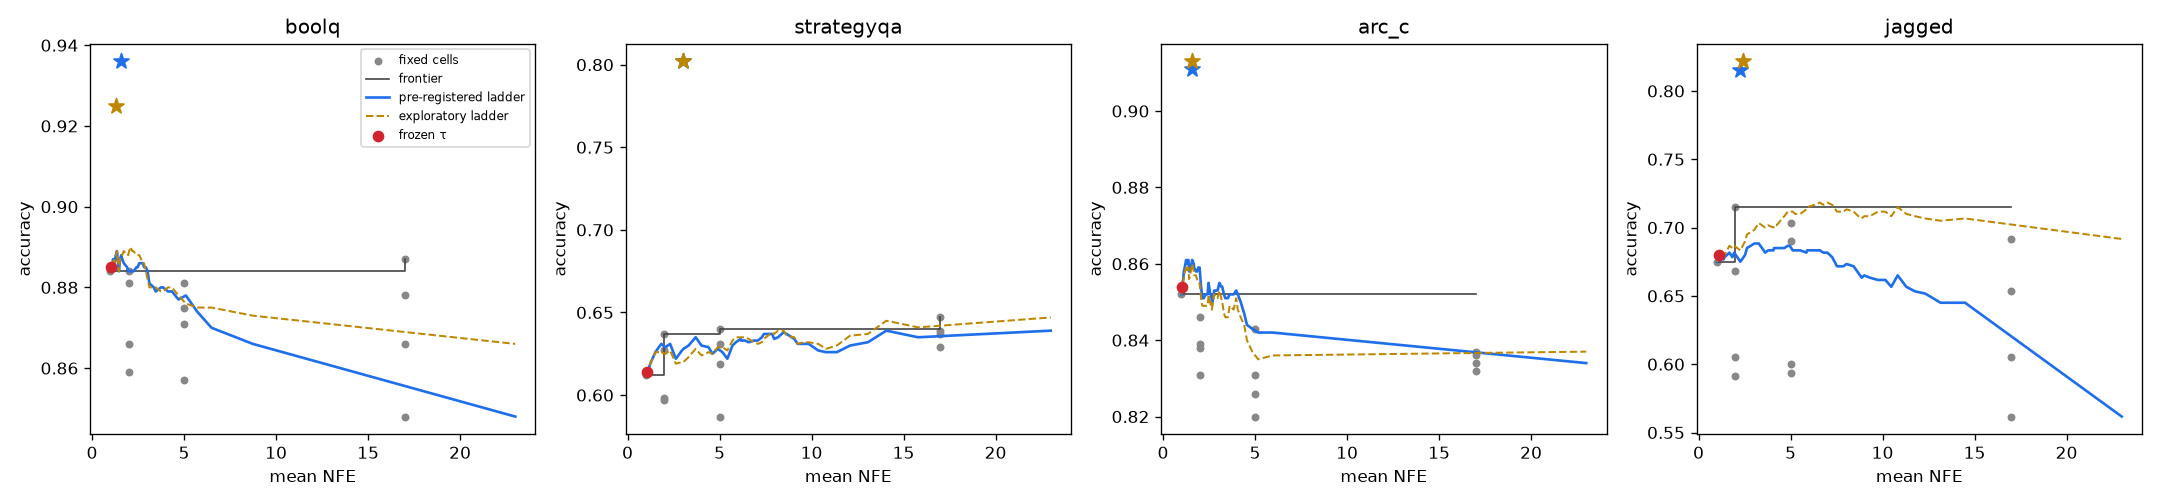
\includegraphics[width=\linewidth]{figs/accuracy_vs_nfe_test.png}
\caption{Accuracy against mean NFE for LLaDA-8B-Instruct on the full test set: fixed cells, the running-maximum frontier, both escalation ladders, the frozen-$\tau$ point, and the oracle. The escalation curves stay at or near the frontier and do not dominate it on any dataset.}
\label{fig:acc_nfe}
\end{figure}

\begin{figure}[h!]
\centering
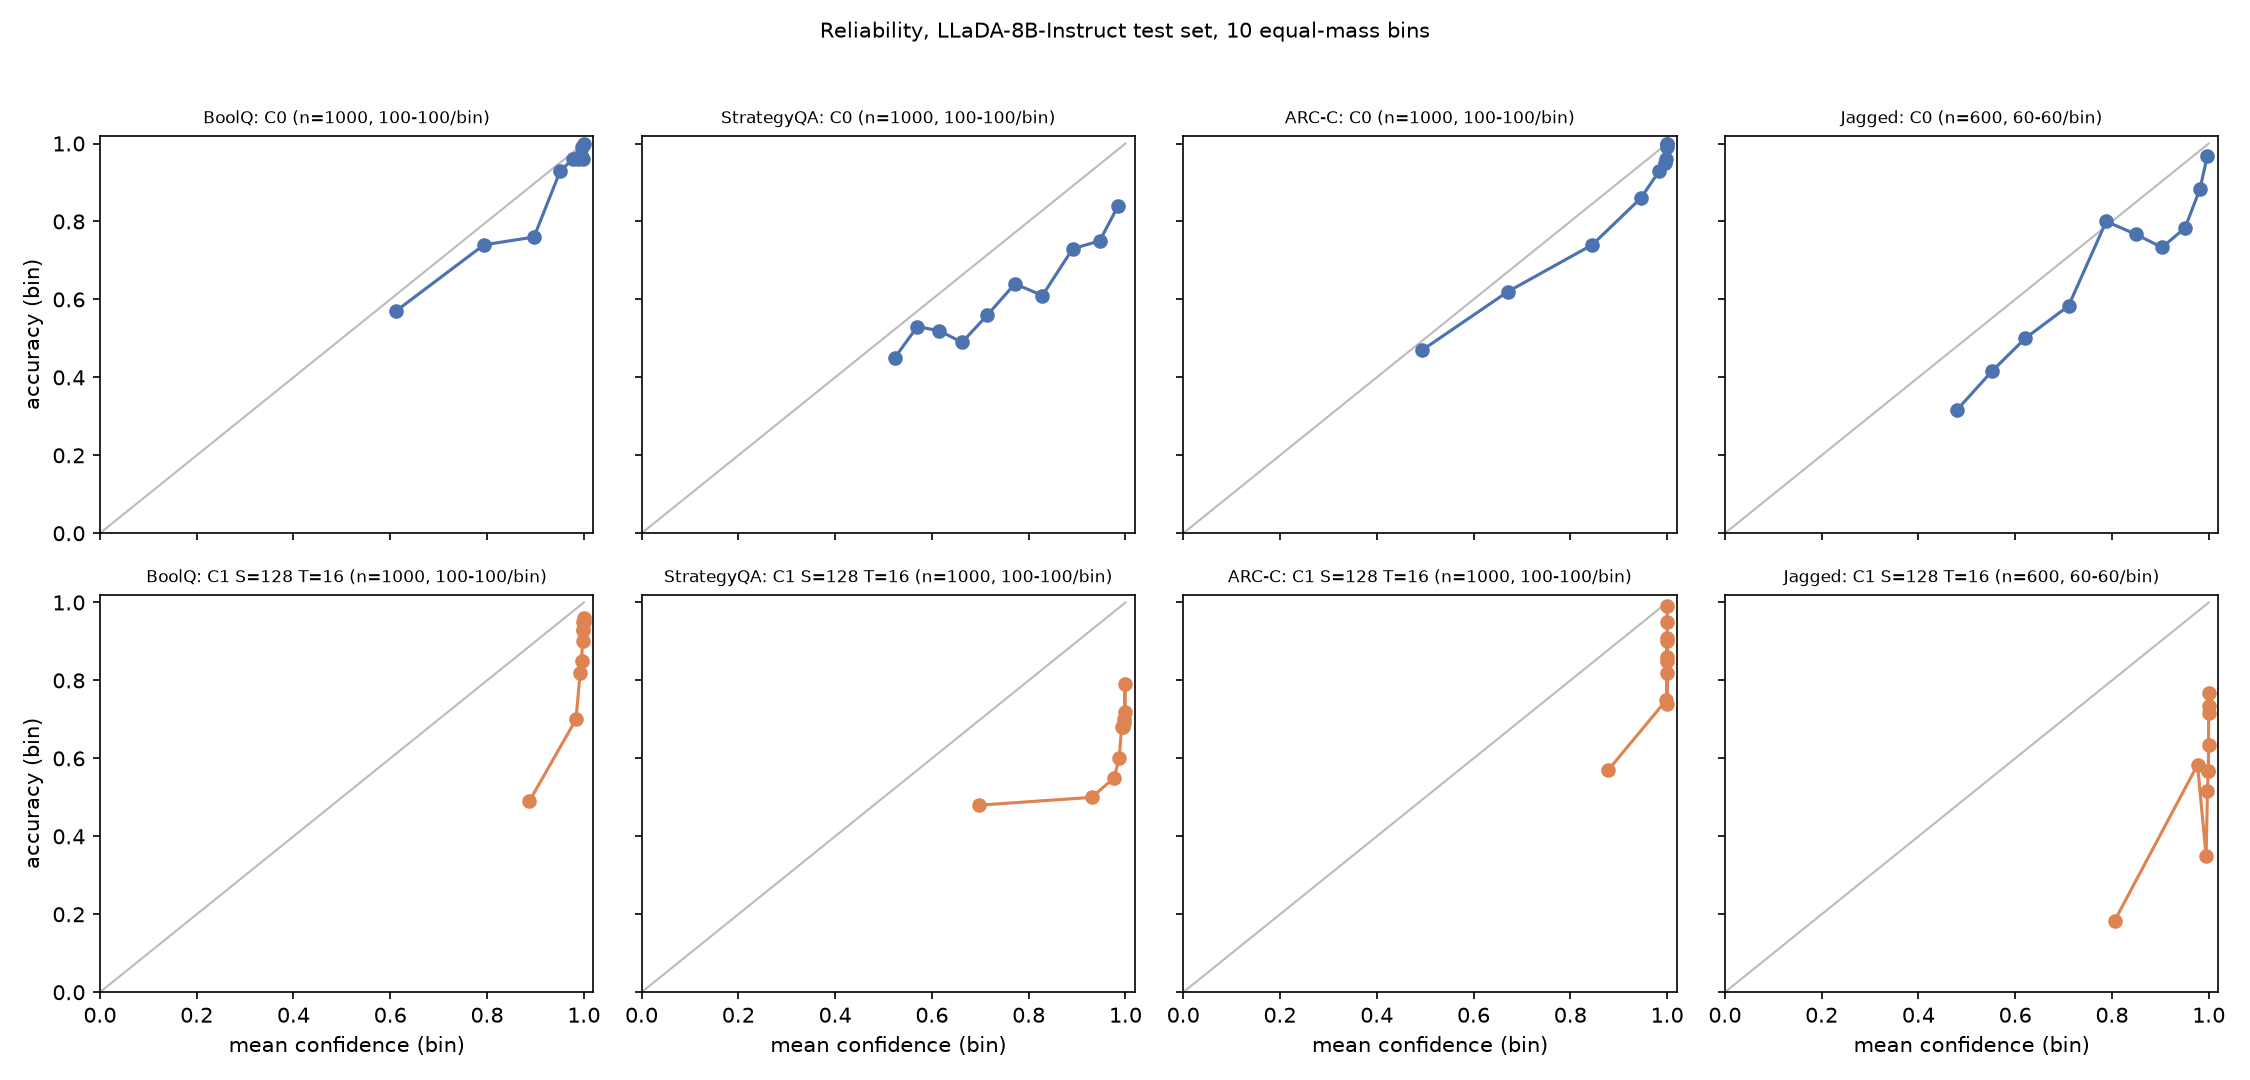
\includegraphics[width=\linewidth]{figs/reliability_equal_mass.png}
\caption{Reliability diagrams for LLaDA-8B-Instruct on the full test set, C0 (top) and C1($S{=}128,T{=}16$) (bottom), using 10 equal-mass bins (so no bin is sparse; bin sizes are printed in each panel title). On every dataset the mean gap between bin confidence and bin accuracy is larger for C1 than for C0, matching its higher ECE.}
\label{fig:reliability}
\end{figure}

\begin{figure}[h!]
\centering
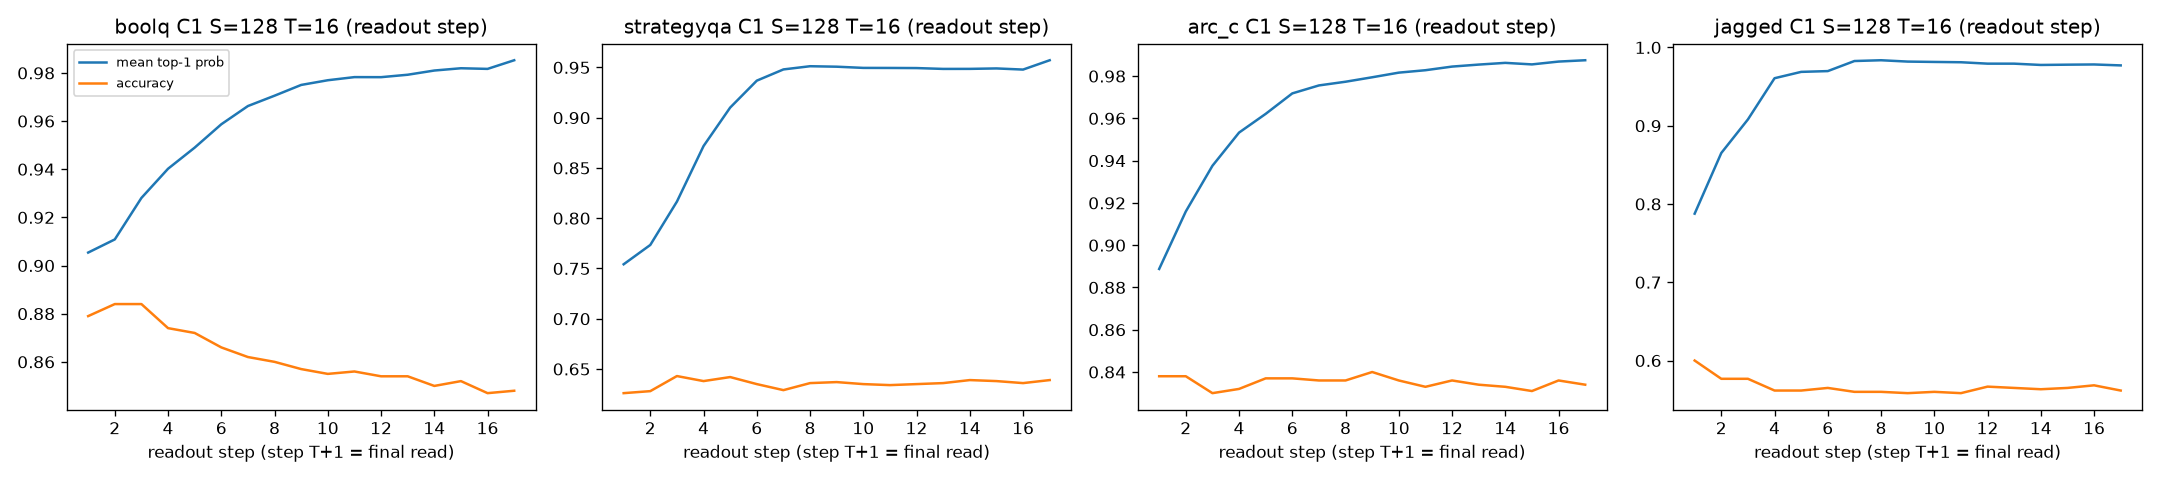
\includegraphics[width=\linewidth]{figs/anytime_test.png}
\caption{Anytime readouts for LLaDA-8B-Instruct C1($S{=}128,T{=}16$) on the full test set: mean top-1 probability and accuracy of the answer slot at each readout step. Mean top-1 probability rises from 0.754 to 0.905 at the first readout to 0.957 to 0.988 at the final read, while accuracy changes by at most 0.038.}
\label{fig:anytime}
\end{figure}

\end{document}
